\documentclass[11pt, oneside]{article}   	% use "amsart" instead of "article" for AMSLaTeX format
\usepackage{geometry}                		% See geometry.pdf to learn the layout options. There are lots.
\geometry{letterpaper}                   		% ... or a4paper or a5paper or ...
%\geometry{landscape}                		% Activate for rotated page geometry
%\usepackage[parfill]{parskip}    		% Activate to begin paragraphs with an empty line rather than an indent
\usepackage{graphicx}				% Use pdf, png, jpg, or eps§ with pdflatex; use eps in DVI mode
								% TeX will automatically convert eps --> pdf in pdflatex
								\usepackage[bb=boondox]{mathalfa}
\usepackage{mathtools}
\usepackage{amssymb}
\usepackage{amsmath,amsfonts,amsthm} % Math packages
\usepackage{bm}
\usepackage{graphicx}
\usepackage{dsfont}
\graphicspath{ {images/} }

%SetFonts

%SetFonts

\DeclareMathOperator*{\argmin}{arg\,min}
\DeclareMathOperator*{\argmax}{arg\,max}
\newcommand{\horrule}[1]{\rule{\linewidth}{#1}} % Create horizontal rule command with 1 argument of height

\title{
\normalfont \normalsize
\textsc{14D006 Stochastic Models and Optimization} \\ [25pt] % Your university, school and/or department name(s)
\horrule{0.5pt} \\[0.4cm] % Thin top horizontal rule
\huge Play Selection in American Football\\ % The assignment title
\horrule{2pt} \\[0.5cm] % Thick bottom horizontal rule
}

\author{Daniel Bestard, Michael Cameron, Hans-Peter H{\"o}llwirth, Akhil Lohia} % Your name

\date{\normalsize\today} % Today's date or a custom date

\begin{document}
\maketitle

%%%%%%%%
% Motivation %
%%%%%%%%
\section{Motivation}
In the following sections we assume some basic understanding of the American football rules.


%%%%%%%%%%%%
% The Football Model %
%%%%%%%%%%%%
\section{The Football Model}
In our American football model we consider the score of one offense drive and add to it the expected points gained by the opposing team from our final field position. More concretely, we want to maximize the expected difference between our drive-score and the opposing team's responding drive-score (which is simply a function of our final field position). \\\\
The state of the system $i \in S$ is described by a vector of 3 quantities: $i = [x,y,d]$:
\begin{itemize}
\item x = the number of yards to the goal (discrete value between 1 and 100)
\item y = the number of yards to go until the next first down (discrete value between 1 and 100)
\item d = down number ($\in \{1,2,3,4\}$)
\end{itemize}
At each state, the team can choose from one of 4 play options (actions) $u \in U$ with $U=\{R, P, U, K\}$:
\begin{itemize}
\item (R)un: moves $D_p - 2$ yards forward with $D_p \sim \text{Poisson}(6)$ 
\item (P)ass: moves $D_p - 2$ yards forward with $D_p \sim \text{Poisson}(12)$ 
\item P(u)nt: moves $6 D_p  + 6$ yards forward with $D_p \sim \text{Poisson}(10)$ 
\item (K)ick: successful with probability $\max(0, .95 - .95x/60)$
\end{itemize}
The set of state-action pairs determine the stationary policy $\mu$. The reward of the drive is determined by the final state transition:
\begin{itemize}
\item Touchdown: 6.8 points (from run or pass) 
\item Opponent's touchdown: -6.8 points (from run or pass)
\item Safety: -2.0 points (from pass or run)
\item Field goal: 3.0 points (from kick)
\item No score due to fumble (from run), interception (from pass), missed 4th down (from pass or run), missed field-goal (from kick) or punt
\end{itemize}
Fixed probabilities are assigned to the outcome of each action.

%%%%%%%%%%%%%%%%%%%%
% Dynamic Programming Formulation %
%%%%%%%%%%%%%%%%%%%%
\newpage
\section{Dynamic Programming Formulation}

\subsection{Optimal Solution}

\subsection{Approximation with Neuro-Dynamic Programming}

%%%%%%%%
% Simulation %
%%%%%%%%
\section{Simulation}
The approximations of the reward-to-go function $J_{u_k}(i^*)$ are obtained from simulated sample trajectories. The simulation routine takes as inputs a policy $\mu$ and a starting state $i^*$ and then generates $N$ sample drives. Each generated sample drive represents a realization of the following probabilistic model (probabilities in brackets):
\begin{itemize}
\item (R)un attempts result in either
\begin{itemize}
\item (0.05) fumble
\item (0.95) run with movement $D_r -2$ with $D_r \sim \text{Poisson}(6)$
\end{itemize}
\item (P)ass attempts result in either
\begin{itemize}
\item (0.05) pass interception with movement $D_p -2$ with $D_p \sim \text{Poisson}(12)$
\item (0.05) sack with movement $D_s$ with $D_s \sim \text{Poisson}(6)$
\item (0.45) pass incomplete
\item (0.45) pass complete with movement $D_p -2$ with $D_p \sim \text{Poisson}(12)$
\end{itemize}
\item P(U)nt attempts always result in turn-over with movement $6 D_p + 6$ with $D_p \sim \text{Poisson}(10)$ 
\item (K)ick attempts result in either
\begin{itemize}
\item (max(0,(0.95-0.95x/60)) successful field goal
\item (otherwise) missed field goal
\end{itemize}
\end{itemize}

The drive terminates in any of the following events:

The simulation returns $N$ sample drives. Each drive $l$ is described by its status sequence $(i_t^l)$ for $t=1,...,T^l$ and reward $g_{T^i}^l$.

\subsection{Expected Reward}
Given a set of $N$ simulated sample trajectories for a specific policy $\mu$, we can estimate the expected reward of this policy from a starting state $i^*$:
$$
\widetilde{J}_{u_k}(i^*) = \frac{1}{N}\sum_{l=1}^N g_{T^i}^l
$$
where $g_{T^i}^i$ denotes the reward of the $i^{th}$ sample trajectory with drive length $T^i$.

\subsection{Heuristic Benchmark}
Rhe simulations and the expected reward function can be used to yield a heuristic benchmark for the optimal play-selection policy. We use the suggested heuristic policies from the paper in order to establish the correctness of the simulation algorithm. In particular, we consider the following heuristic policies:
\begin{enumerate}
\item If $d=1$ (first down): (\textbf{P})ass

\item If $d=2$ (second down): 
\begin{enumerate}
\item If $y<3$ (less than 3 yards to next first down): (\textbf{R})un
\item If $y\geq3$ (3 or more yards to next first down): (\textbf{P})ass
\end{enumerate}

\item If $d=3$ (third down): 
\begin{enumerate}
\item If $x<41$ (less than 41 yards to goal):
\begin{enumerate}
\item If $y<3$ (less than 3 yards to next first down): (\textbf{P})ass or (R)un
\item If $y\geq3$ (3 or more yards to next first down): (\textbf{P})ass or (R)un
\end{enumerate}
\item If $x \geq 41$ (less than 41 yards to goal):
\begin{enumerate}
\item If $y<3$ (less than 3 yards to next first down): (P)ass or (\textbf{R})un
\item If $y\geq3$ (3 or more yards to next first down): (\textbf{P})ass or (R)un
\end{enumerate}
\end{enumerate}

\item If $d=4$ (forth down): 
\begin{enumerate}
\item If $x<41$ (less than 41 yards to goal):
\begin{enumerate}
\item If $y<3$ (less than 3 yards to next first down): (P)ass or (\textbf{R})un or (K)ick
\item If $y\geq3$ (3 or more yards to next first down): (P)ass or (R)un or (\textbf{K})ick
\end{enumerate}
\item If $x \geq 41$ (less than 41 yards to goal):
\begin{enumerate}
\item If $y<3$ (less than 3 yards to next first down): (P)ass or (\textbf{R})un or P(U)nt
\item If $y\geq3$ (3 or more yards to next first down): (P)ass or (R)un or P(\textbf{U})nt
\end{enumerate}
\end{enumerate}

\end{enumerate}

We estimated the expected reward for each of the $2^4*3^4 = 1296$ heuristic policy combinations from starting position $i^* = (x=80, y=10, d=1)$ (one of the most likely starting positions in football) and found the best heuristic expected reward-to-go $J_{\mu}(i^*) = -1.26$. The associated policy to this reward is highlighted in bold. Note that the reward-to-go matches the heuristic result of the underlying paper, thus establishing the correctness of the simulation algorithm.

%%%%%%%%%
% API and OPI %
%%%%%%%%%
\section{Approximate and Optimistic Policy Iteration}



\subsection{Multilayer Perceptron (MLP)}

\begin{figure}[ht!]
\centering
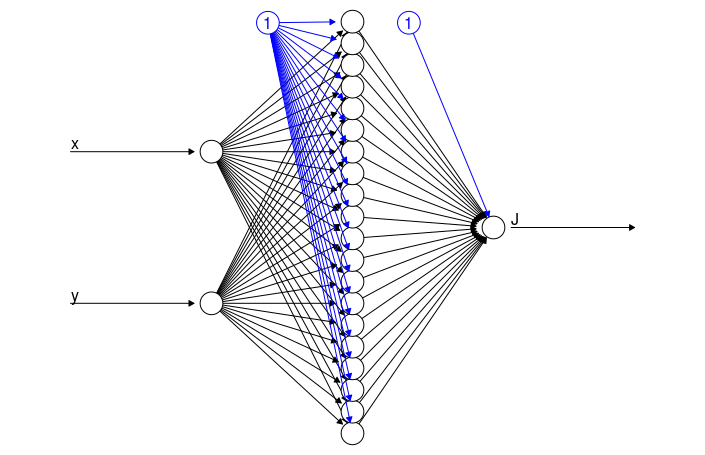
\includegraphics[width=155mm]{../images/neuralnet.png}
\caption{Architecture of neural network with one hidden layer ($R=20$ nodes)}
\end{figure}

\subsection{Policy Update}

%%%%%%
% Results %
%%%%%%
\section{Results}

\end{document}















